\documentclass[a4paper,11pt]{article}
\usepackage[margin=20mm]{geometry}
\usepackage{graphicx,booktabs,hyperref}
\begin{document}
\title{PM12 CFD simulator DAC characterization}
\author{FIT hardware acceptance bench}
\date{10 November 2026}\maketitle
\section{Identification and connections}
Board: PM12-K7-3A17A1B402212223 (previous FPGA DNA identification).
MCU EEPROM serial 1803 was checked in this session.
Four CFD simulators occupy physical PM channels 12, 10, 8 and 6.
Their analog monitor outputs share one measurement bus. Only one MAX4051
monitor output is enabled at a time. All four monitors are inhibited between
transfer curves and on exit. Other GPIO controls are preserved.

Instrument: Keysight B2910BL, serial MY63320299. The monitor bus connects to
Force HI/LO; Sense is unconnected. Local (2-wire) voltage measurement is used,
with a current source setting of 0 A, 1 microampere source range,
6 V compliance, 20 V measurement range and 1 PLC integration.
OUTP is enabled during measurement; automatic output-on is disabled.
OUTP OFF/high impedance is restored on exit. The owner explicitly confirmed
Force wiring and authorized 0 A/OUTP ON operation.
\section{Procedure and scope}
The remaining channels 10, 8 and 6 are scanned. DAC B is observed through
DRV\_OFFSET (monitor 3), DAC C through CFD\_OFFSET (monitor 0), and DAC D
through CFD\_CMP\_OFFSET (monitor 1). Phase DAC A is unchanged.
The resistor networks produce decreasing spans of approximately 40 mV for B
and 20 mV for C, and an increasing span of approximately 1.06 V for D.

Each DAC is scanned over 101 rounded integer codes spanning 0--65535, with
three fresh READ? samples per code and 100 ms settling after each write.
Compliance, protection and overflow bits are checked. Raw status words and
timestamps are retained; unspecified status bits are ignored per the Keysight
SCPI reference, Table 1-2. Each exercised DAC is explicitly set to 0000 on exit.
STORED firmware parameters are not treated as active hardware readback.

This is a functional DC transfer scan, not exhaustive 16-bit INL/DNL or a
calibrated accuracy certificate. Three repeats estimate short-term scatter.
No independent calibrated reference was available; freshness was checked by
switching between the 1.3 V rail and DRV\_VOCM on channel 12.
\section{Measured endpoint summary}
\begin{center}\begin{tabular}{rr rrr r}\toprule
PM ch. & DAC & Code 0 (V) & Code 65535 (V) & Span (V) & Max. $s$ ($\mu$V)\\\midrule
10 & B & 1.044730 & 1.004507 & -0.040223 & 68.1 \\
8 & B & 1.044680 & 1.004540 & -0.040140 & 60.3 \\
6 & B & 1.045580 & 1.005527 & -0.040053 & 49.3 \\
10 & C & 1.034757 & 1.014360 & -0.020397 & 76.4 \\
8 & C & 1.034793 & 1.014350 & -0.020443 & 66.6 \\
6 & C & 1.035827 & 1.015247 & -0.020580 & 56.9 \\
10 & D & 0.004743 & 1.069480 & 1.064737 & 55.1 \\
8 & D & 0.005847 & 1.066383 & 1.060537 & 69.3 \\
6 & D & 0.005947 & 1.066433 & 1.060487 & 60.0 \\
\bottomrule\end{tabular}\end{center}
\clearpage
\section{Transfer curves}
\begin{center}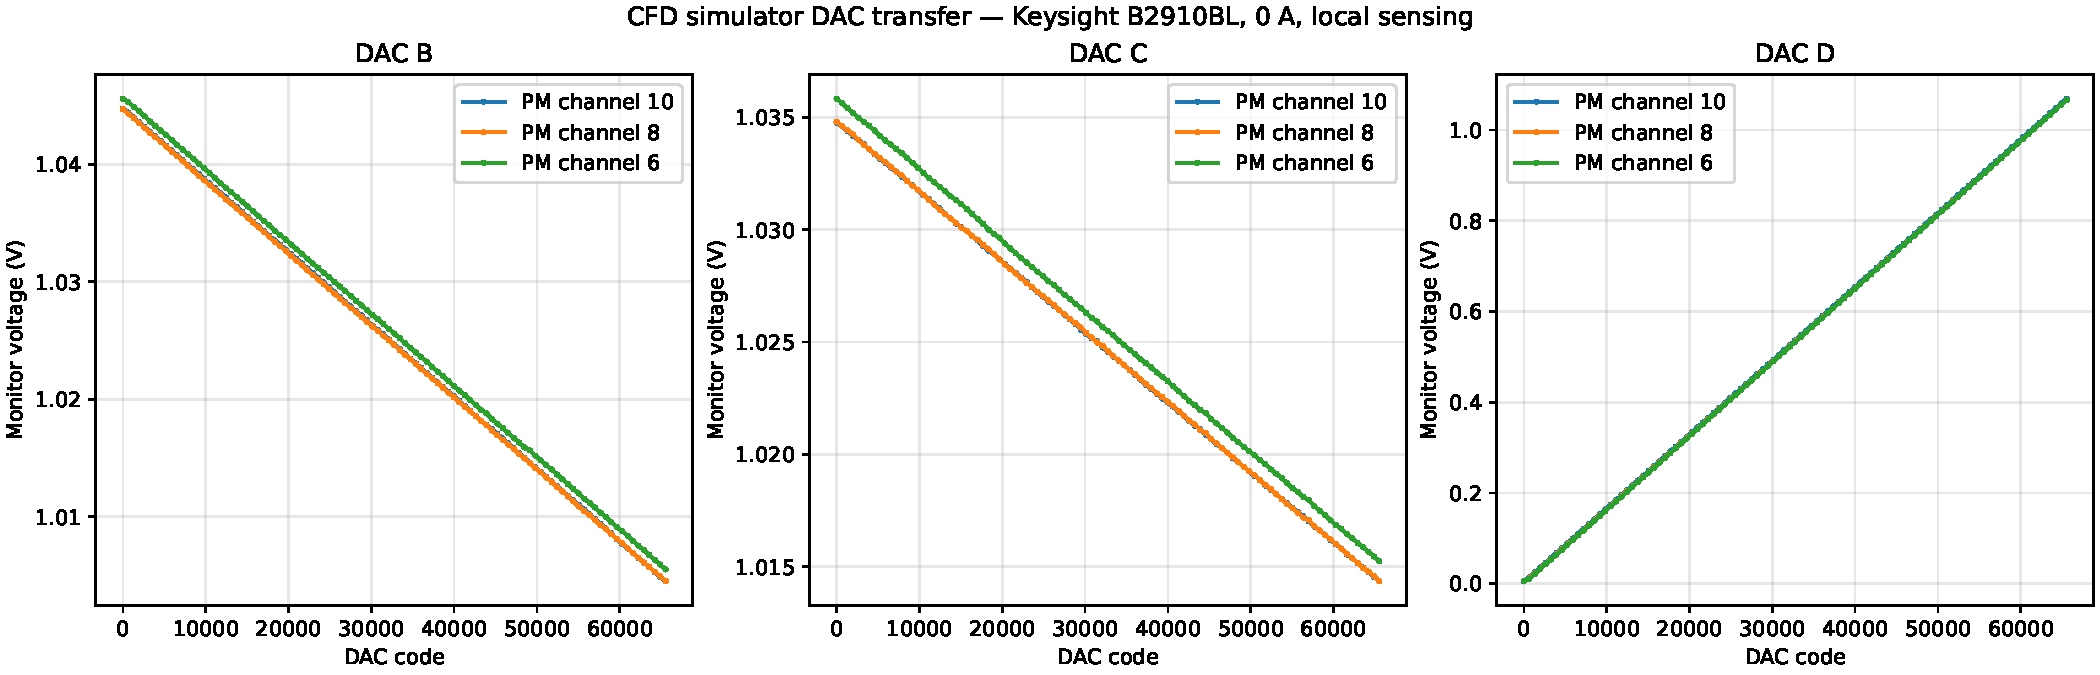
\includegraphics[width=\textwidth]{dac-transfer.pdf}\end{center}
The physical channels are overlaid for each DAC.
\begin{center}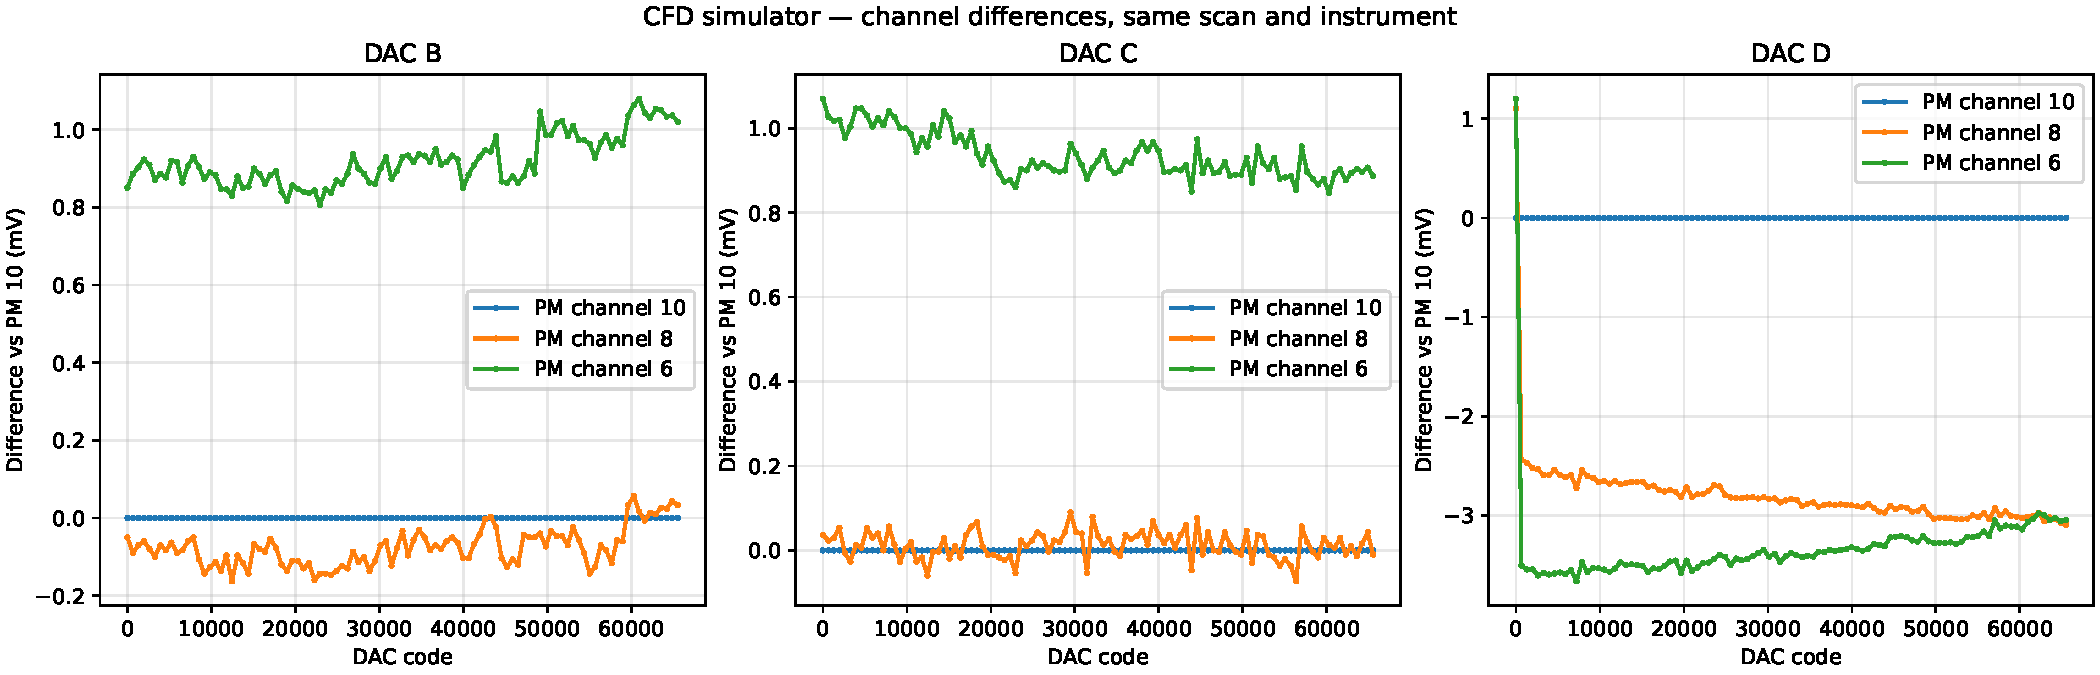
\includegraphics[width=\textwidth]{dac-channel-differences.pdf}\end{center}
Differences use channel 10 as reference within the same run.
\clearpage
\section{Gain and lower endpoint behavior}
All nine curves are monotonic on the sampled grid. Gain is fitted over
5--95\% of the code range and compared with the nominal DAC/resistor scaling.
The gain deviations below characterize the complete analog chain.
The zero-code residual compares the measured minimum-code voltage with the
extrapolated interior fit. DAC D shows a distinct lower-end departure;
this scan alone does not locate its cause within the DAC and analog stages.
\begin{center}\begin{tabular}{rr rr}\toprule
PM ch. & DAC & Interior gain error (\%) & Zero-code residual (mV)\\\midrule
10 & B & 0.226 & -0.066 \\
8 & B & 0.016 & 0.008 \\
6 & B & -0.177 & -0.047 \\
10 & C & -0.055 & -0.051 \\
8 & C & -0.047 & -0.028 \\
6 & C & 0.612 & 0.019 \\
10 & D & 0.034 & 1.406 \\
8 & D & -0.013 & 5.096 \\
6 & D & 0.086 & 6.261 \\
\bottomrule\end{tabular}\end{center}
\section{Evidence and final state}
Raw samples: \texttt{samples.csv}. Statistics: \texttt{summary.csv/json}.
Commands, I2C readbacks, restoration receipts, instrument identity and final
state: \texttt{scan-report.json}. Completeness and status checks are in
\texttt{validation.json}; their PASS is not a calibrated analog acceptance limit.
Figures: \texttt{plot\_smu\_dacs.py}; editable chapter:
\texttt{report\_smu\_dacs.py}.
\paragraph{Acquisition completed:} True.
\paragraph{Final SMU output:} 0 (0 means OFF).
All nine DAC restoration receipts confirm raw code 0000. Final mux inhibition
and disconnected upstream TCA masks are checked before releasing the leases.
\end{document}
